\documentclass[]{article}

% Imported Packages
%------------------------------------------------------------------------------
\usepackage{amssymb}
\usepackage{amstext}
\usepackage{amsthm}
\usepackage{amsmath}
\usepackage{enumerate}
\usepackage{fancyhdr}
\usepackage[margin=1in]{geometry}
\usepackage{graphicx}
\usepackage{extarrows}
\usepackage{setspace}
\usepackage{float}
\usepackage{vhistory}
%------------------------------------------------------------------------------

% Header and Footer
%------------------------------------------------------------------------------
\pagestyle{plain}  
\renewcommand\headrulewidth{0.4pt}                                      
\renewcommand\footrulewidth{0.4pt}                                    
%------------------------------------------------------------------------------

% Title Details
%------------------------------------------------------------------------------
\title{Deliverable \#3 Template}
\author{SE 3A04: Software Design II -- Large System Design}
\date{}                               
%------------------------------------------------------------------------------

% Document
%------------------------------------------------------------------------------
\begin{document}
	
	\maketitle	
	
	\section{Introduction}
	\label{sec:introduction}
	
	\subsection{Purpose}
	\label{sec:purpose}
	
	The purpose of this document is to give a detailed design of the software architecture of the WhoDatDog mobile application. This document is provide detailed figures and diagrams of the complete software structure of the application. The diagrams contained in the document visually describe how the classes within the system will interact with one another. This document is intended for use by software design and system support personnel.
	
	\subsection{System Description}
	\label{sec:sysdescription}
	
	The WhoDatDog system is a mobile application developed for mobile devices running a Google Android operating system of version 8.4.2 or higher. This system's primary function is to enable a user to identify the breed of a dog they may find in their immediate, physical environment. Additionally, the system enables users to search for locations where they may purchase or adopt a dog in their vicinity, i.e. pet stores, dog pounds, etc., and to create posts on the Twitter social network, to describe to other users a dog they have identified and the geographic location where they have seen it.\\\\In order to accomplish these functions, the WhoDatDog software system employs a hierarchical system architecture which includes user interfaces at the top level, system controllers at the bottom level, and system memory at the lower level. In particular, the system's memory contains three so-called "expert" systems which are used for dog breed identification, and the system also uses external systems in the form of Twitter and Google Maps plugins.
	
	\subsection{Overview}
	\label{sec:overview}
	
	The contents of this document are organized into 5 sections, including Section 1, the introduction. Sections 2-4 contain diagrams showing the software structure and interactions between components.\\Section 2 contains state charts for controller classes, which show all the possible scenarios when using the application and how the system will behave when performing a certain operation.\\Section 3 contains sequence diagrams, which shows the interactions between different classes within the system in a time sequence format and the result the system has when an interaction has been done.\\Section 4 contains detailed class diagrams, contained is a figure of all the components of the WhoDatDog application as well as how each component interacts with others in the system.\\Though it does not describe the system, Section 5 states the division of labor among the authors of this document.

% End SubSection

% End Section

\section{State Charts for Controller Classes}
\label{sec:state_charts_for_controller_classes}

\begin{figure}[H]
	\centering
	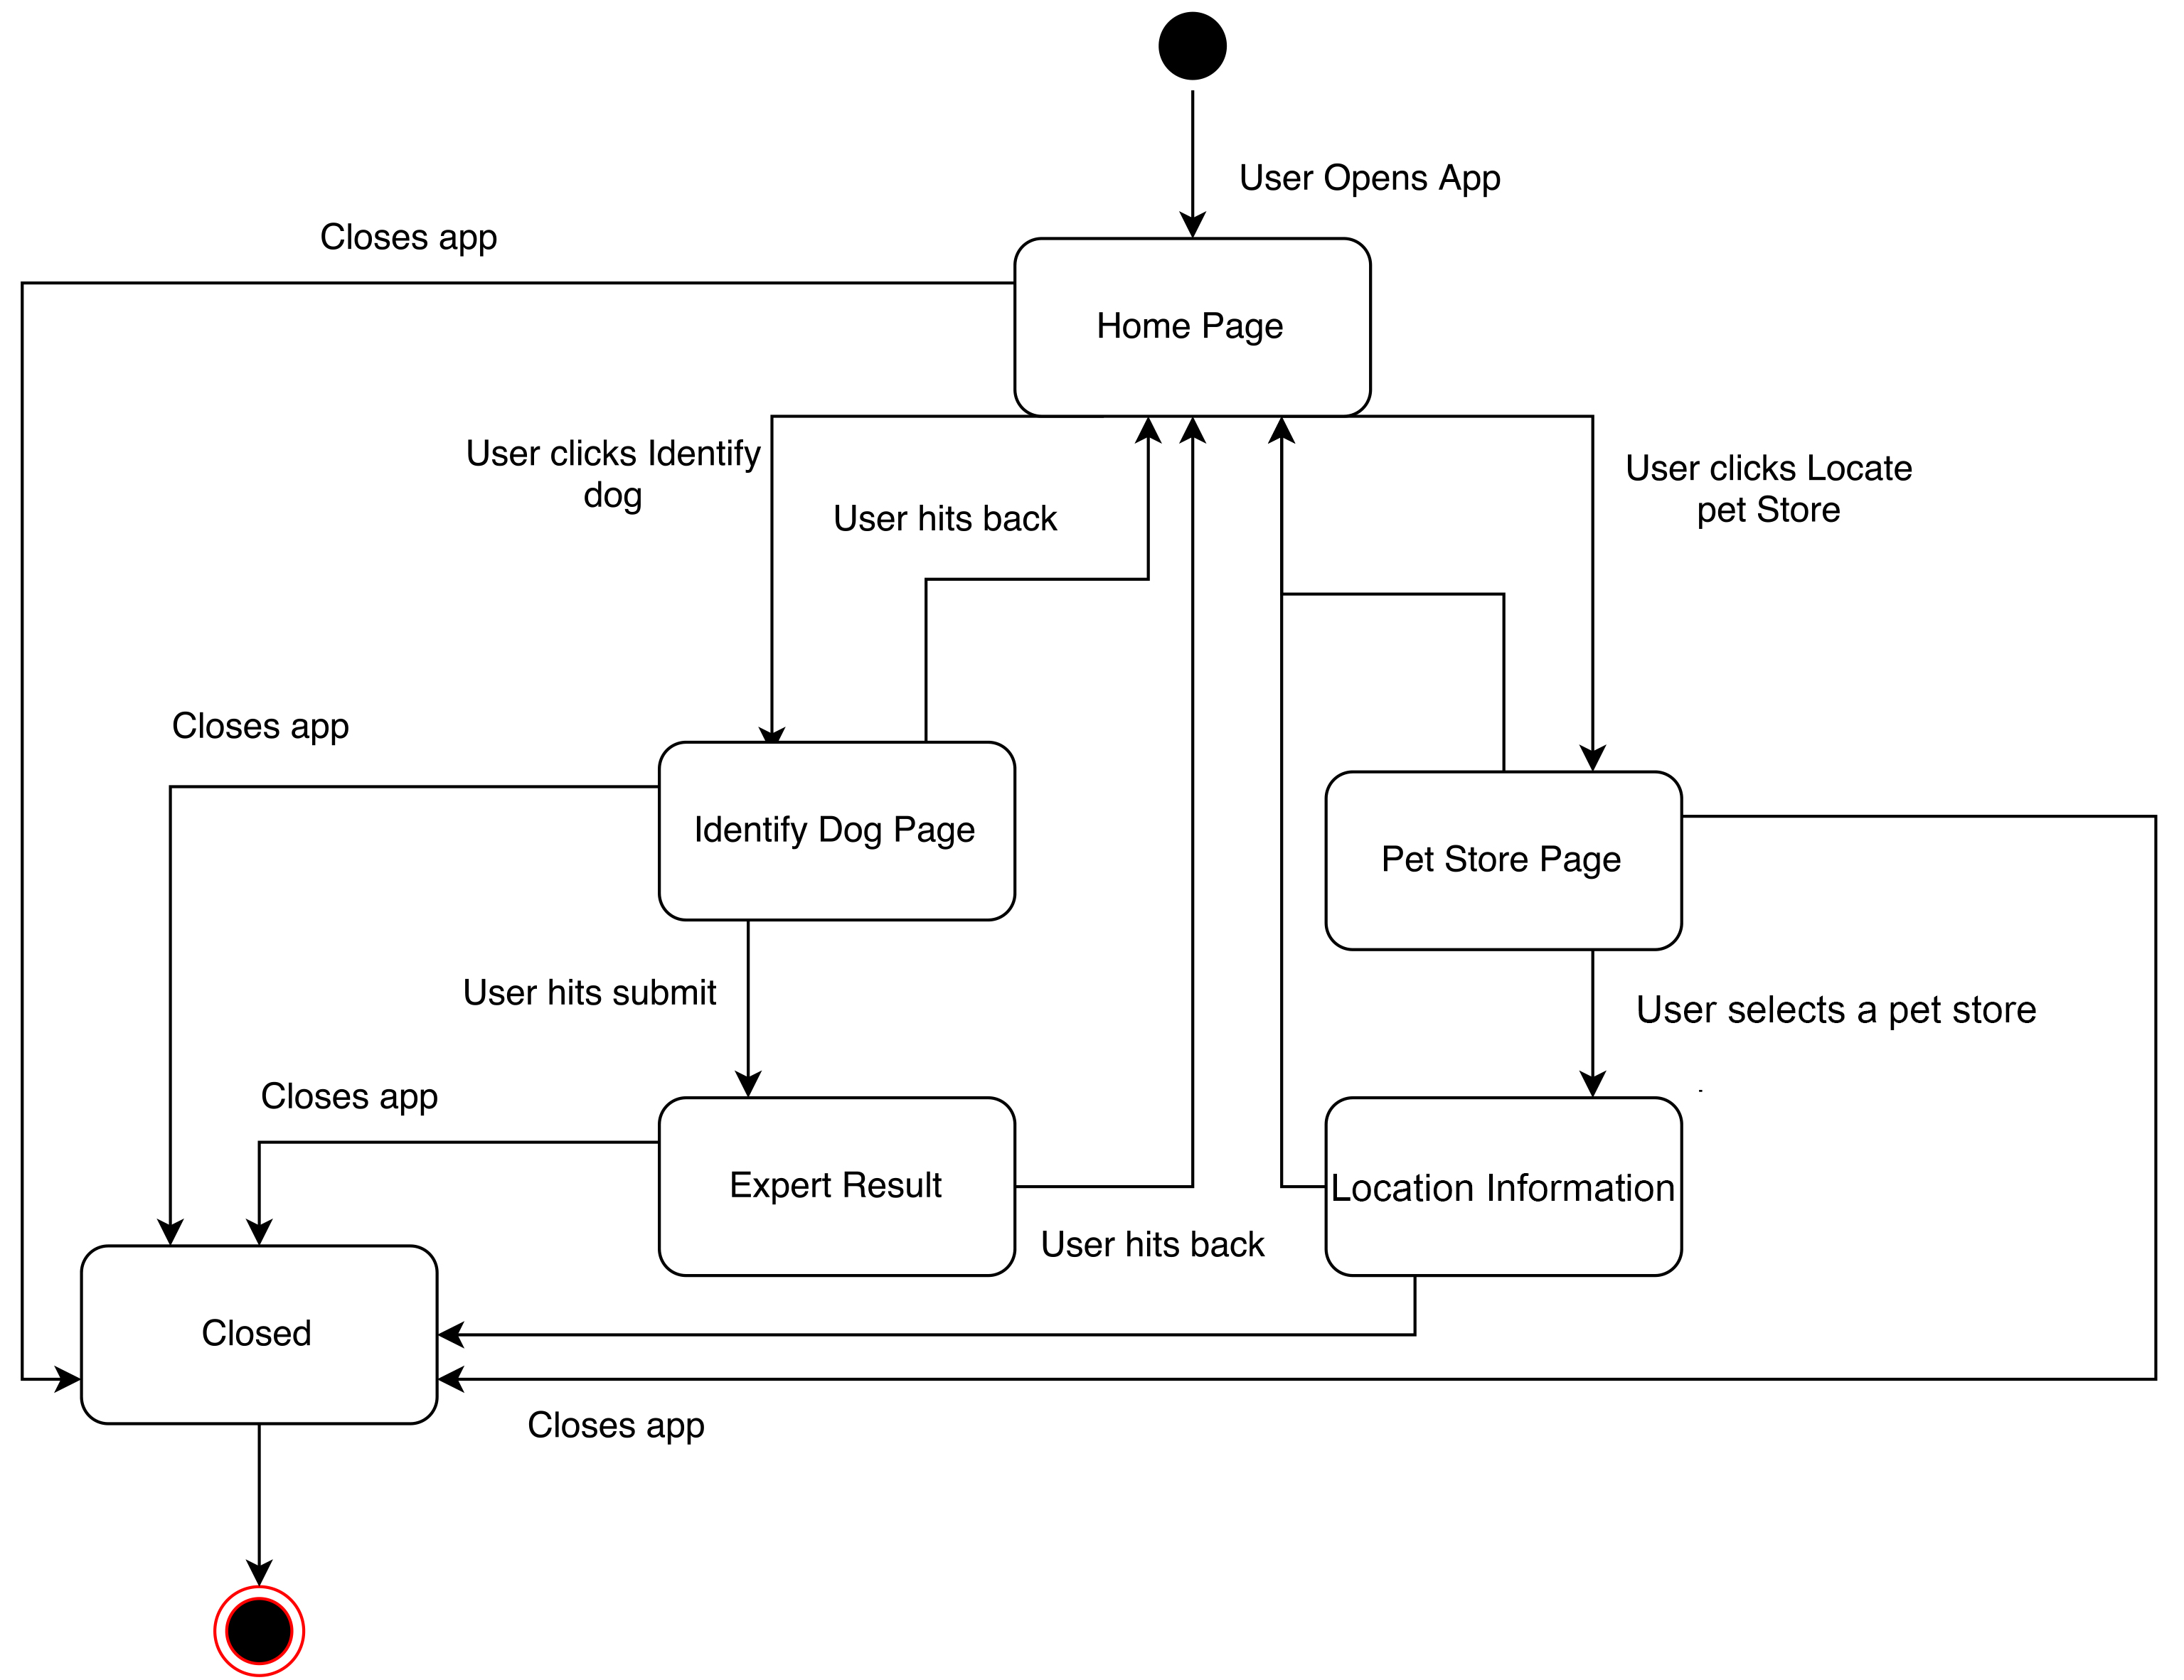
\includegraphics[width=\textwidth]{ForumController.jpg}
	\caption{\label{fig:analysisclassdiagram}The state chart of the Forum Controller of the WhoDatDog system.}
\end{figure}

\begin{figure}[H]
	\centering
	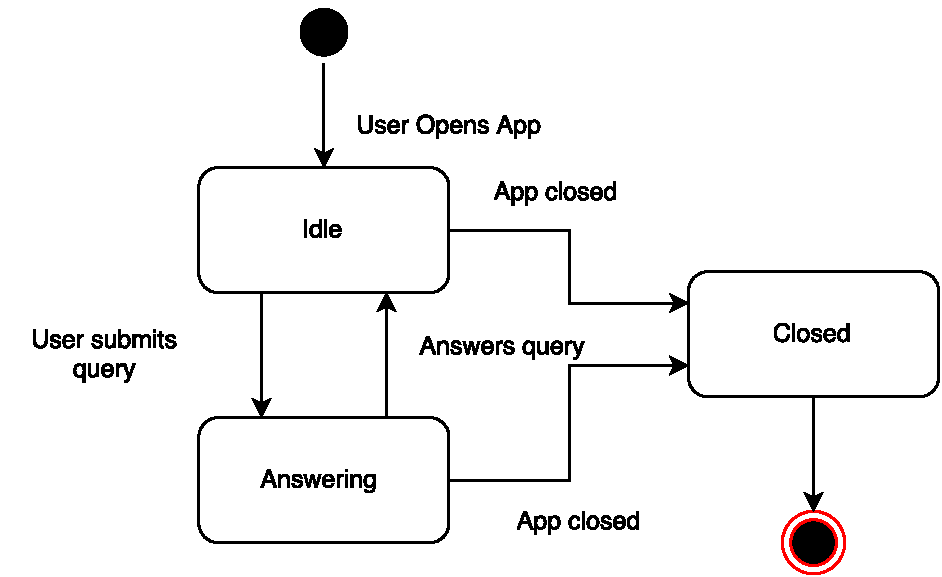
\includegraphics[width=\textwidth]{ExpertController.pdf}
	\caption{\label{fig:analysisclassdiagram}The state chart of the Expert Controller of the WhoDatDog system.}
\end{figure}

There will be at least  5 Expert Controller but they will have the same state chart



\begin{figure}[H]
	\centering
	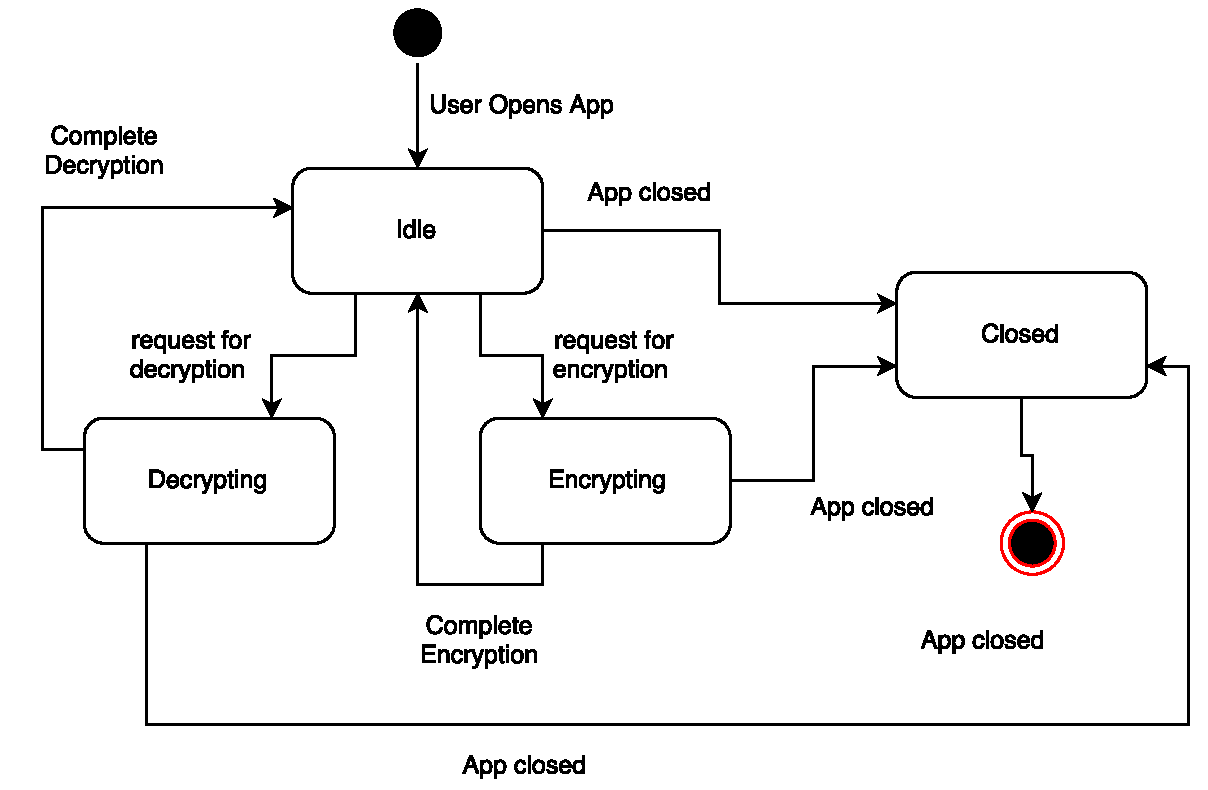
\includegraphics[width=\textwidth]{EncryptionController.pdf}
	\caption{\label{fig:analysisclassdiagram}The state chart of the Encryption Controller of the WhoDatDog system.}
\end{figure}


\begin{figure}[H]
	\centering
	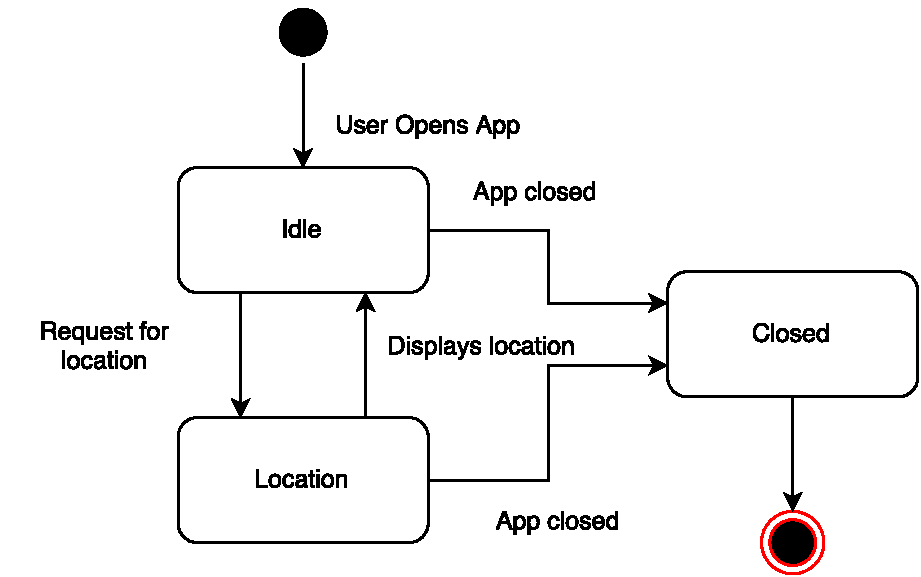
\includegraphics[width=\textwidth]{GoogleMapsController.pdf}
	\caption{\label{fig:analysisclassdiagram}The state chart of the Google Maps Controller of the WhoDatDog system.}
\end{figure}


\begin{figure}[H]
	\centering
	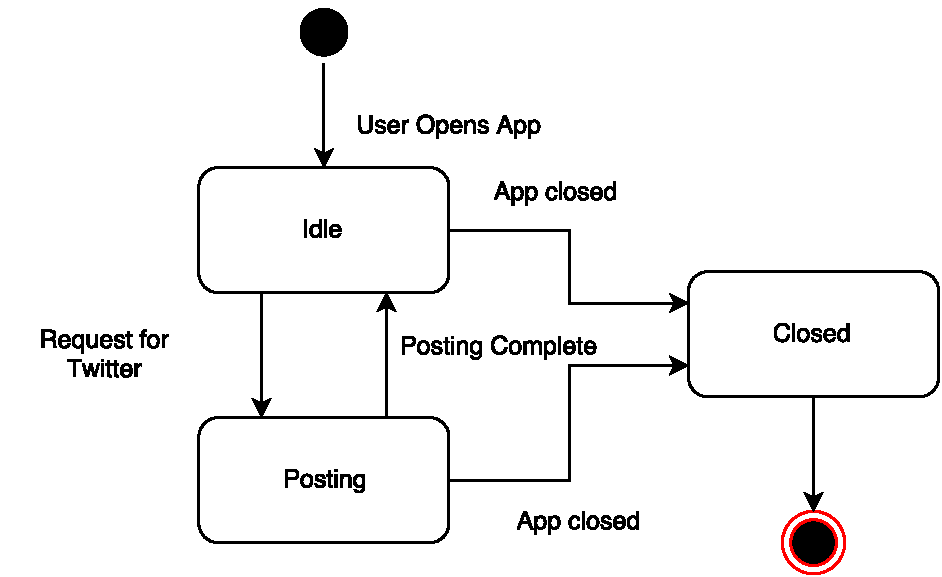
\includegraphics[width=\textwidth]{TwitterController.pdf}
	\caption{\label{fig:analysisclassdiagram}The state chart of the Twitter Controller of the WhoDatDog system.}
\end{figure}




\section{Sequence Diagrams}
\label{sec:sequence_diagrams}
\begin{figure}[H]
	\centering
	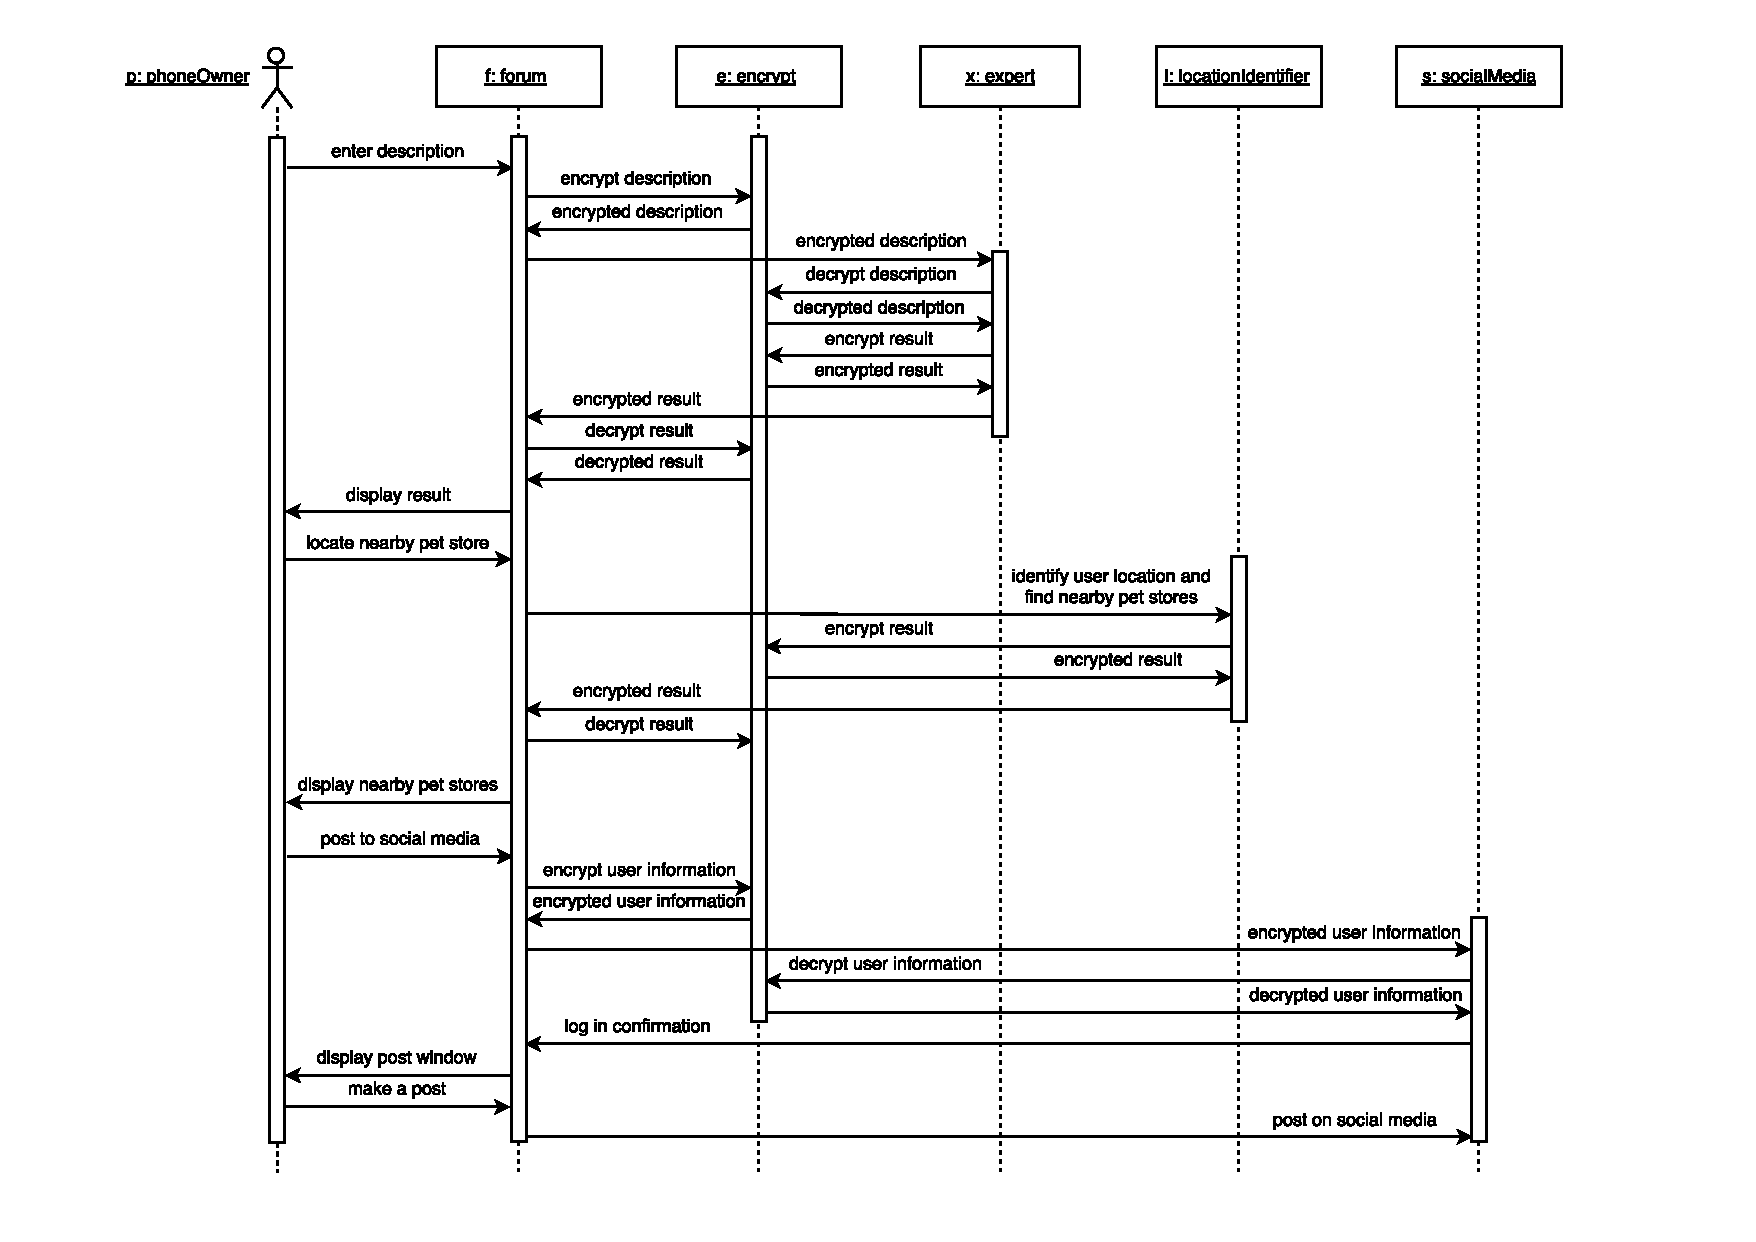
\includegraphics[width=\textwidth]{sequencediagram.pdf}
	\caption{\label{fig:analysisclassdiagram}The sequence diagram of the WhoDatDog system.}
\end{figure}

\section{Detailed Class Diagram}

\begin{figure}[H]
	\centering
	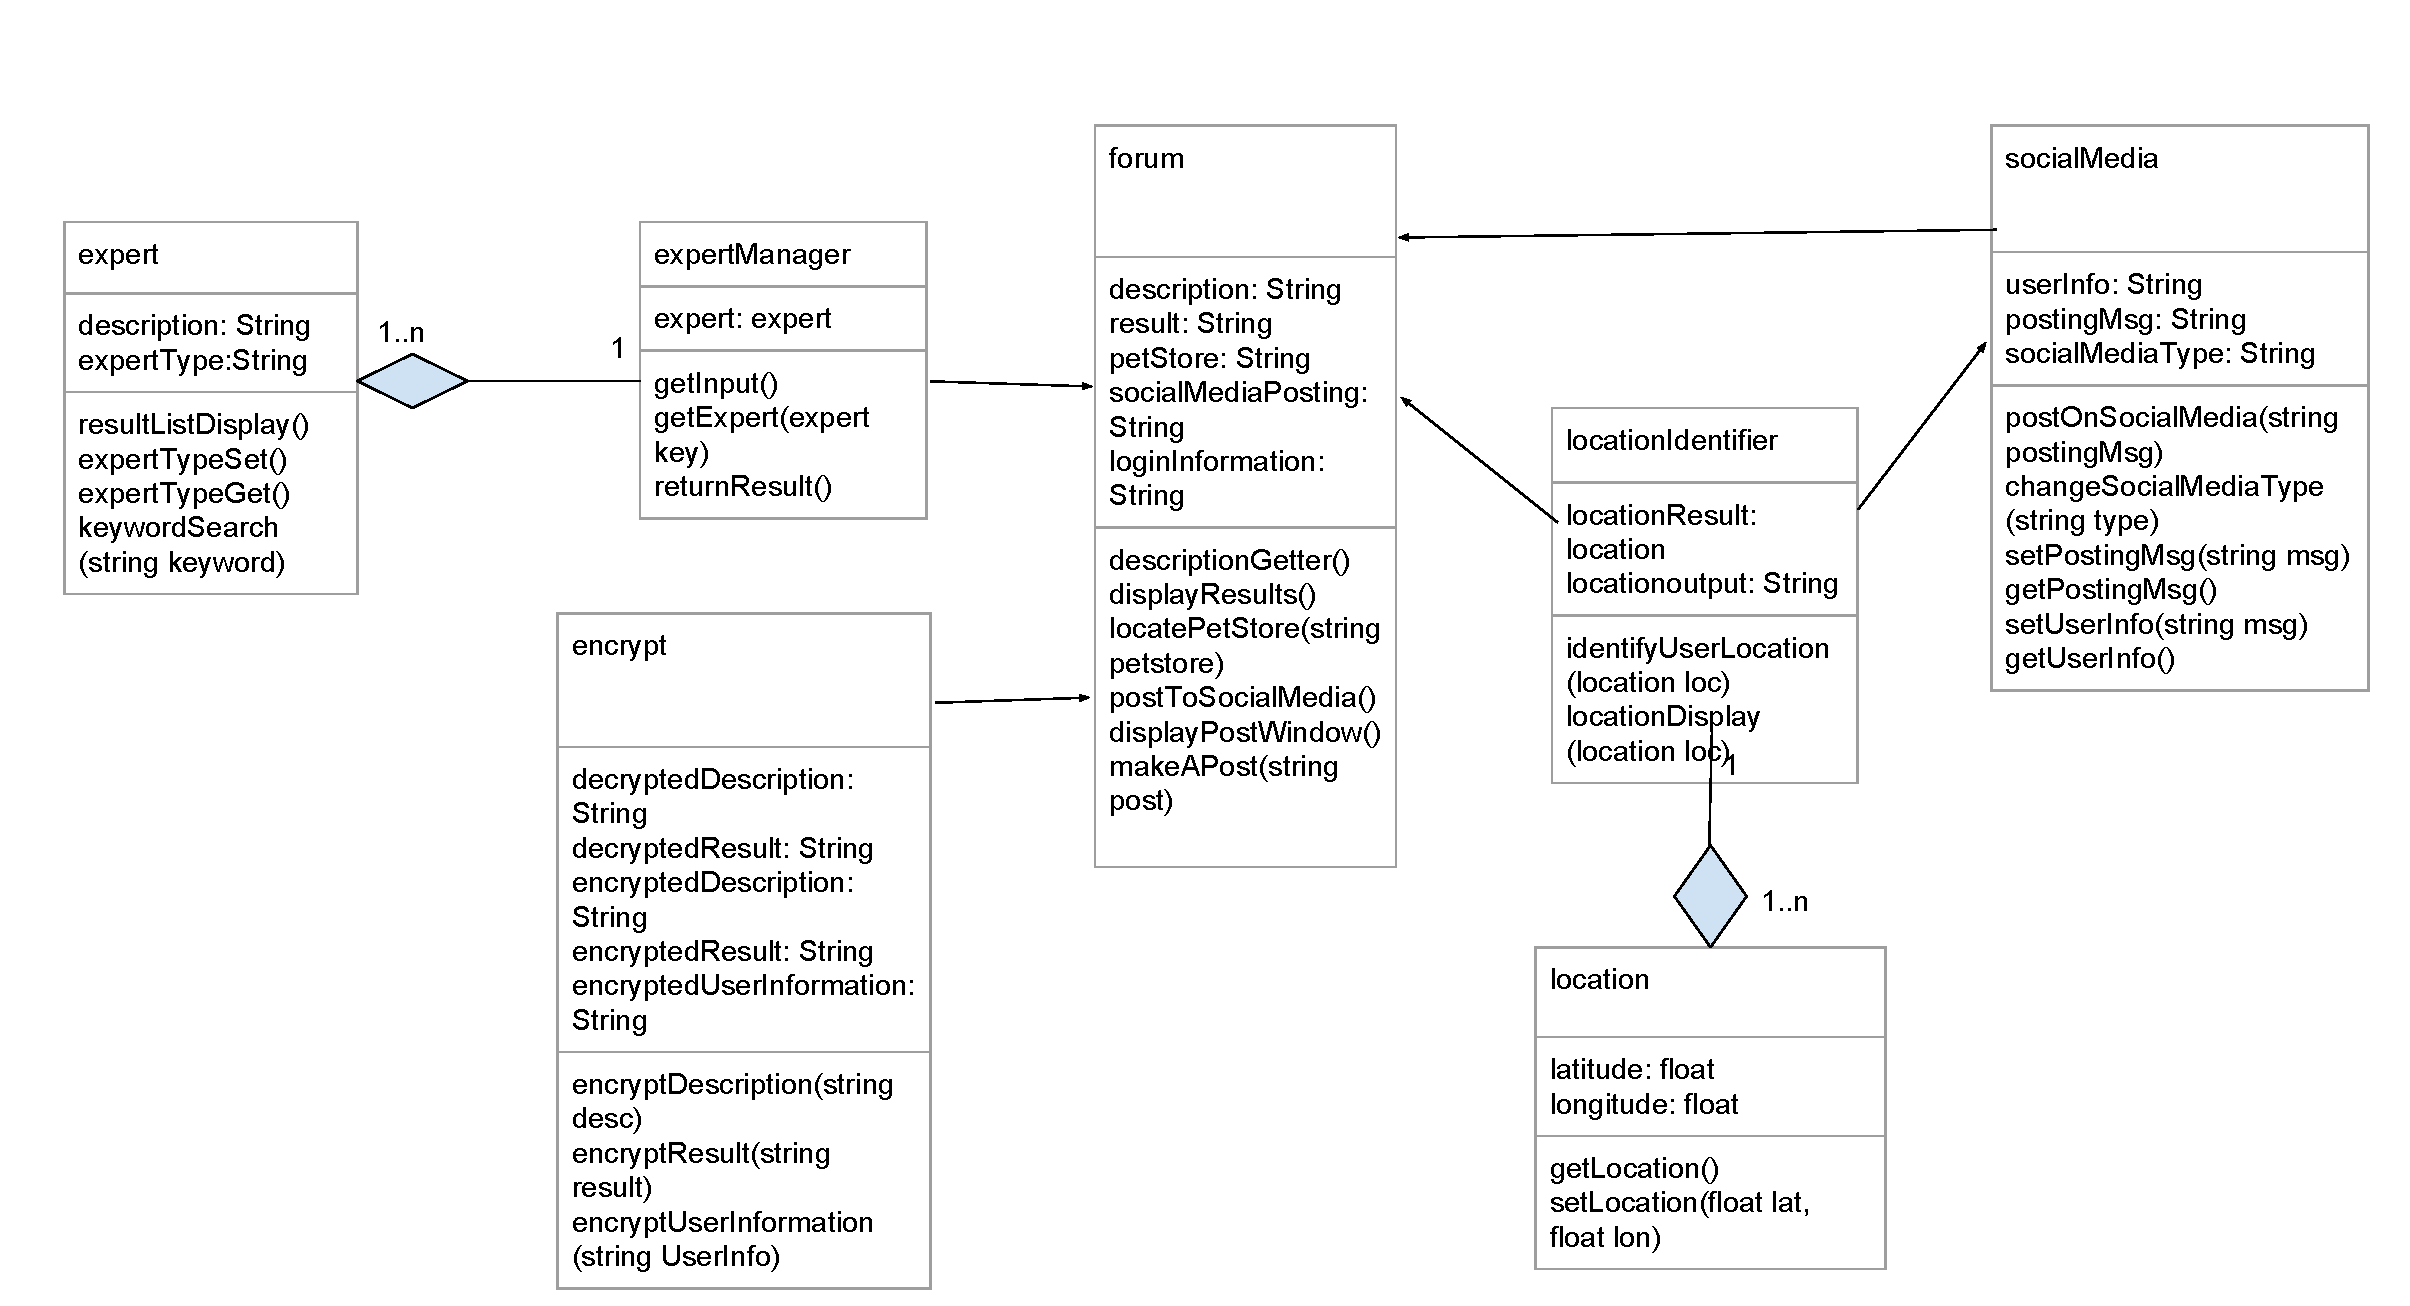
\includegraphics[width=\textwidth]{DetailClassDiagram.pdf}
	\caption{\label{fig:analysisclassdiagram}The Detailed Class diagram of the WhoDatDog system.}
\end{figure}

\appendix
\section{Division of Labour}


test

\newpage
--------------------------------------------------------